% !TEX program = xelatex
\documentclass[12pt,a4paper]{ctexart}

% ======================
% Packages
% ======================
\usepackage{geometry}
\usepackage{graphicx}
\usepackage{xcolor}
\usepackage{amsmath, amssymb}
\usepackage{array}
\usepackage{booktabs}
\usepackage{tabularx}
\usepackage{setspace}
\usepackage{titlesec}
\usepackage{fancyhdr}
\usepackage{float}
\usepackage{tikz}
\usetikzlibrary{positioning,arrows.meta,shapes.geometric,shapes.symbols,fit,backgrounds,calc}
\usepackage{tcolorbox}
\tcbuselibrary{listings, breakable}
\usepackage{enumitem}
\newcolumntype{L}[1]{>{\raggedright\arraybackslash}p{#1}}
\newcolumntype{C}[1]{>{\centering\arraybackslash}p{#1}}
\newcolumntype{R}[1]{>{\raggedleft\arraybackslash}p{#1}}



\usepackage[colorlinks=true, linkcolor=black, citecolor=green, urlcolor=cyan]{hyperref}
% ======================
% 页面设置
% ======================
\geometry{a4paper,left=2.5cm,right=2.5cm,top=2.5cm,bottom=2.5cm}
\setlength{\headheight}{15pt}
\setstretch{1.3}

% ======================
% 颜色
% ======================
\definecolor{titleblue}{RGB}{65,105,225}
\definecolor{darkgreen}{RGB}{0,120,70}
\definecolor{highlight}{RGB}{200,30,30}

% ======================
% 标题样式
% ======================
\titleformat{\section}
{\Large\bfseries\color{titleblue}}
{\thesection}{1em}{}

\titleformat{\subsection}
{\large\bfseries\color{darkgreen}}
{\thesubsection}{1em}{}

% ======================
% 页眉页脚
% ======================
\pagestyle{fancy}
\fancyhf{}
\fancyhead[L]{VeriAgent Project}
\fancyhead[R]{智能技术工程实训}
\fancyfoot[C]{\thepage}

\begin{document}

% ==================================================
% 封面
% ==================================================

\begin{figure}[htbp]
    \centering
    
\includegraphics[width=0.45\textwidth]{media/dhu.png}
\end{figure}

\vspace{1cm}

\begin{center}

{\Huge\bfseries\color{titleblue}人工智能应用实践系统实现报告}

\vspace{0.8cm}

{\LARGE\bfseries 面向招聘场景的智能人才评估与推荐平台}

\vspace{0.4cm}



\end{center}

\vspace{2cm}

\begin{center}

\begin{minipage}{0.75\textwidth}

\renewcommand{\arraystretch}{2.2}

\begin{tabular}{>{\bfseries\large}l >{\large}l}

组\quad 员： & 郑吴穷 \quad 于笑 \quad 李汉尧 \\

学\quad 号： & 231380128 \quad 231380124 \quad 220820114 \\

学\quad 院： & 信息与智能科学学院 \\

专\quad 业： & 智能科学与技术 \\

课程名称： & 智能技术工程实训 \\

报告类型： & 系统实现报告 \\

日期： & 2026/4/6\\

\end{tabular}

\end{minipage}

\end{center}

\vfill

\begin{center}

东华大学

信息与智能科学学院

\end{center}

\newpage

% ==================================================
% 目录
% ==================================================
\setcounter{tocdepth}{2}
\tableofcontents
\newpage

% ==================================================
% 第一章 系统概述
% ==================================================
\section{系统概述}

ScoutAgent 是一个面向猎头与企业招聘场景的\textbf{智能人才审计与评估平台}。系统以「企业 $\to$ 岗位 $\to$ 投递 $\to$ 评估」为主线业务流，通过多个 AI Agent 对候选人简历进行结构化解析、岗位匹配、真实性核查和深度对话评估，辅助招聘决策者高效、精准地完成人才甄别。

\subsection*{核心价值主张}

\begin{itemize}[itemsep=4pt]
  \item 用大语言模型将非结构化简历 PDF 转化为结构化知识节点；
  \item 用知识图谱（Neo4j）消除技能名称歧义，提升跨语言、跨表述的匹配准确度；
  \item 用多轮对话式深度评估替代粗糙的简历评分，还原真实的岗位适配度判断；
  \item 构建长期候选人画像，沉淀每一次交互的信息价值。
\end{itemize}

% ==================================================
% 第二章 系统功能结构
% ==================================================
\section{系统功能结构}

从\textbf{用户与业务视角}对系统进行功能划分，与智能体分层架构图、数据模型 ER 图侧重点不同：本节约束在「用户能完成哪些任务」及模块之间的依赖关系。

\begin{figure}[H]
\centering
\begin{tikzpicture}[
  font=\small,
  >=Stealth,
  mod/.style={draw, rounded corners=4pt, minimum width=3.0cm, minimum height=0.78cm,
              align=center, fill=blue!8},
  sub/.style={draw, rounded corners=3pt, minimum width=2.65cm, minimum height=0.58cm,
              align=center, fill=green!6, font=\footnotesize},
  root/.style={draw, rounded corners=5pt, minimum width=3.9cm, minimum height=0.88cm,
               align=center, fill=blue!18, font=\bfseries\small},
  arr/.style={->, thick, color=gray!55},
]
\node[root] (r) {ScoutAgent\\核心功能域};

\node[mod, below left=1.05cm and 0.15cm of r] (m1) {用户鉴权};
\node[mod, below=1.05cm of r] (m2) {企业与岗位};
\node[mod, below right=1.05cm and 0.15cm of r] (m3) {候选人库};

\node[mod, below left=1.05cm and 0.75cm of m2] (m4) {评估看板};
\node[mod, below right=1.05cm and 0.75cm of m2] (m5) {评估助手};

\node[sub, below=0.52cm of m1] (s1) {登录 / JWT 会话};
\node[sub, below=0.52cm of m2] (s2) {企业 / JD / 投递};
\node[sub, below=0.52cm of m3] (s3) {简历 / 解析 / 投递记录};
\node[sub, below=0.52cm of m4] (s4) {批量匹配 / 真实性};
\node[sub, below=0.52cm of m5] (s5) {SSE 多轮对话};

\draw[arr] (r) -- (m1);
\draw[arr] (r) -- (m2);
\draw[arr] (r) -- (m3);
\draw[arr] (m2) -- (m4);
\draw[arr] (m2) -- (m5);
\end{tikzpicture}
\caption{系统功能结构（用户视角）}
\label{fig:functional-structure}
\end{figure}

典型依赖关系：用户须先完成\textbf{鉴权}；在\textbf{企业与岗位}模块维护企业与岗位并产生投递；\textbf{候选人库}负责简历上传与解析；\textbf{评估看板}对选中投递批量触发 JD-CV 匹配与真实性评估；\textbf{评估助手}在单投递维度提供深度对话式分析。

\subsection{系统技术架构总览}

图~\ref{fig:system-tech} 汇总浏览器、API、智能体与外部依赖在一页内的拓扑关系，可与第~\ref{sec:agents}~节智能体细化设计、第~\ref{sec:techstack}~节技术栈表对照阅读。

\begin{figure}[H]
\centering
\begin{tikzpicture}[
  font=\small, >=Stealth,
  client/.style={draw, rounded corners=4pt, fill=blue!7, minimum width=2.3cm, align=center},
  api/.style={draw, rounded corners=4pt, fill=orange!12, minimum width=2.9cm, align=center},
  agent/.style={draw, rounded corners=4pt, fill=green!9, minimum width=7.2cm, minimum height=0.85cm, align=center},
  data/.style={draw, rounded corners=4pt, fill=blue!5, minimum width=2.35cm, align=center},
  ext/.style={draw, rounded corners=4pt, fill=purple!10, minimum width=2.35cm, align=center},
  arr/.style={->, thick, color=gray!60},
]
\node[client] (fe) at (0,0) {浏览器\\React SPA};
\node[api] (be) at (4.2,0) {FastAPI\\REST / SSE};
\node[agent] (ag) at (4.2,-1.9)
  {智能体层：简历解析 · JD-CV 匹配 · 真实性 · LangGraph 对话};
\node[data] (pg) at (1.2,-3.7) {PostgreSQL};
\node[data] (neo) at (4.2,-3.7) {Neo4j};
\node[ext] (llm) at (7.2,-3.7) {LLM API\\（OpenAI 兼容）};

\draw[arr] (fe) -- node[above,font=\tiny]{HTTPS} (be);
\draw[arr] (be) -- (ag);
\draw[arr] (ag) -- (pg);
\draw[arr] (ag) -- (neo);
\draw[arr] (ag) -- (llm);
\end{tikzpicture}
\caption{系统技术架构总览（端到端）}
\label{fig:system-tech}
\end{figure}

% ==================================================
% 第三章 智能体设计
% ==================================================
\section{智能体设计}\label{sec:agents}

\subsection{整体架构}

图~\ref{fig:arch} 展示了 ScoutAgent 的整体智能体架构。按\textbf{业务功能}划分：\textbf{（1）简历解析与案例解析}同属一条能力线——上传简历后由\textbf{简历解析 Agent} 将 PDF 等解析为结构化数据，并在候选人库中形成可检索、可展示的「候选人案例」视图；\textbf{（2）岗位与投递}为另一条能力线——在企业/岗位工作台维护企业与 JD、创建投递（含上传简历生成候选人并投递）；\textbf{（3）评估与深度对话}中，\textbf{评估 Agent} 主要承担 JD-CV 匹配与看板侧\textbf{批量评估}（含真实性打分等）；\textbf{深度对话 Agent} 以多轮对话为主形态，\textbf{知识图谱工具}与\textbf{真实性评估结果}在其链路中作为\textbf{可被调用的工具与上下文}（而非与「对话」并列的另一套主流程）。图中基础设施层的图谱与 LLM 亦由评估侧与对话侧按需共用。技术分层上仍为前端、FastAPI、三类 Agent 及知识图谱 + LLM；所有 LLM 调用均通过 OpenAI 兼容接口，默认模型为 Kimi K2.5，支持通过环境变量切换；主备模型容错由 \texttt{invoke\_with\_fallback} 机制提供。

\begin{figure}[H]
\centering
\begin{tikzpicture}[
  font=\small,
  >=Stealth,
  box/.style={draw, rounded corners=4pt, minimum width=2.8cm, minimum height=0.75cm,
              align=center, fill=white},
  gbox/.style={box, fill=blue!6},
  abox/.style={box, fill=green!8, minimum width=2.4cm},
  tbox/.style={box, fill=orange!10, minimum width=3.6cm},
  layer/.style={draw=gray!50, dashed, rounded corners=6pt, inner sep=8pt},
]

% ── 前端层（与三类业务功能对齐，文字从简） ──
\node[gbox, minimum width=8.4cm, align=center] (fe)
  {前端（React）\\[0.15cm]
   \footnotesize ① 简历解析 / 候选人库 \quad
   ② 岗位与投递 \quad
   ③ 评估看板 / 评估助手};

% ── 后端服务层 ──
\node[gbox, minimum width=8.4cm, below=0.6cm of fe] (be)
  {FastAPI 后端（REST / SSE）};

% ── 三个 Agent ──
\node[abox, below left=0.9cm and 1.4cm of be]  (ra)  {简历解析\\Agent};
\node[abox, below=0.9cm of be]                 (aa)  {评估 Agent\\(JD-CV / 真实性)};
\node[abox, below right=0.9cm and 1.4cm of be] (ca)  {深度对话\\Agent};

% ── 知识图谱工具 ──
\node[tbox, below=1.0cm of aa] (kg)
  {知识图谱工具 \texttt{query\_knowledge\_graph}\\（Neo4j · 同义词 / 分类 / 等价判断）};

% ── LLM ──
\node[tbox, below=0.8cm of kg] (llm)
  {LLM（OpenAI 兼容接口 · Kimi K2.5）\\主备容错 · 温度 / 超时可配};

% ── 箭头 ──
\draw[->] (fe) -- (be) node[midway, right, font=\tiny] {HTTP / SSE};
\draw[->] (be) -- (ra);
\draw[->] (be) -- (aa);
\draw[->] (be) -- (ca);
\draw[->] (aa) -- (kg);
\draw[->] (ca) -- (kg);
\draw[->] (kg) -- (llm);
% 简历解析 Agent → LLM：先垂直到与 LLM 左侧同高，再水平向右进入（左→右），避免折线穿过知识图谱框
\draw[->] (ra.south) -- (ra.south|-llm.west) -- (llm.west);

% ── 分层框 ──
\begin{scope}[on background layer]
  \node[layer, fit=(ra)(aa)(ca), label=above left:{\tiny Agent 层}] {};
  \node[layer, fit=(kg)(llm), label=above left:{\tiny 基础设施层}] {};
\end{scope}

\end{tikzpicture}
\caption{ScoutAgent 整体架构（①②③ 见正文；图谱与真实性评估为深度对话可调用的工具能力）}
\label{fig:arch}
\end{figure}

\subsection{简历实体解析 Agent}

\textbf{目标}：将非结构化简历原文（由 PDF 抽取或直接输入）转化为标准化 JSON 结构，存入数据库 \texttt{cv.parsed\_json} 字段。

图~\ref{fig:resume-flow} 展示了完整的解析调用链路。

\begin{figure}[H]
\centering
\begin{tikzpicture}[
  font=\small, >=Stealth,
  node distance=0.55cm,
  fstep/.style={draw, rounded corners=3pt, fill=blue!6,
               text width=7cm, minimum height=0.7cm, align=center},
  arr/.style={->, thick, color=gray!70},
]
\node[fstep] (s1) {\texttt{POST /api/candidates/\{id\}/cv/parse}};
\node[fstep, below=of s1] (s2) {\texttt{BackgroundTasks} 异步触发解析任务};
\node[fstep, below=of s2] (s3) {\texttt{asyncio.to\_thread} 线程池执行 LLM 调用};
\node[fstep, below=of s3] (s4) {OpenAI SDK 直调（system: 角色+Schema；system: 简历全文；user: 输出规则）};
\node[fstep, below=of s4] (s5) {\texttt{extract\_json\_payload} 解析结构化 JSON};
\node[fstep, below=of s5] (s6) {写入 \texttt{CV.parsed\_json}，回填 \texttt{Candidate} 姓名/邮件/电话};

\draw[arr] (s1)--(s2); \draw[arr] (s2)--(s3);
\draw[arr] (s3)--(s4); \draw[arr] (s4)--(s5);
\draw[arr] (s5)--(s6);
\end{tikzpicture}
\caption{简历实体解析 Agent 调用链路}
\label{fig:resume-flow}
\end{figure}

\textbf{输出 JSON 结构}（关键字段）：

\begin{center}
\renewcommand{\arraystretch}{1.3}
\begin{tabular}{L{3.2cm} L{9cm}}
\toprule
\textbf{字段} & \textbf{说明} \\
\midrule
\texttt{name / email / phone} & 基础联系信息 \\
\texttt{summary} & 个人简介 \\
\texttt{skills} & 技能标签数组 \\
\texttt{work\_experience} & 工作经历列表（公司、职位、时间段、职责要点、成就） \\
\texttt{projects} & 项目经历（名称、描述、技术栈、成果） \\
\texttt{research} & 科研经历（机构、研究方向、成果） \\
\texttt{education} & 教育经历（学校、专业、学位、时间） \\
\bottomrule
\end{tabular}
\end{center}

\textbf{关键设计决策}：使用 OpenAI SDK 直调而非 LangChain，减少抽象层开销，便于精确控制 \texttt{extra\_body}（如 Kimi K2 系列的 thinking 开关）；简历原文以第二条 \texttt{system} 消息传入，避免被模型视为用户指令；解析完成后自动回填候选人基础字段。

解析状态机：\texttt{pending} $\to$ \texttt{parsing} $\to$ \texttt{completed} / \texttt{failed}，前端通过 2 秒轮询感知进度。

% ── JD-CV 匹配 ──
\subsection{JD-CV 匹配 Agent}

\textbf{目标}：综合评估候选人与目标岗位的适配程度，输出结构化评分报告（维度分、总分、优劣势分析）。

图~\ref{fig:jdcv-flow} 展示了匹配 Agent 的工具循环与最终输出逻辑。

\begin{figure}[H]
\centering
\begin{tikzpicture}[
  font=\small, >=Stealth, node distance=0.5cm,
  fstep/.style={draw, rounded corners=3pt, fill=green!7,
               text width=9cm, minimum height=0.68cm, align=center},
  dec/.style={draw, diamond, fill=yellow!15, aspect=3.5,
              text width=4.2cm, align=center, font=\small},
  arr/.style={->, thick, color=gray!70},
]
\node[fstep] (s1) {\texttt{POST /assessments/batch-run}（\texttt{jd\_cv\_match}）};
\node[fstep, below=of s1] (s2) {构建初始消息：SystemMessage（提示词）+ HumanMessage（JD + CV 全文）};
\node[fstep, below=of s2] (s3) {\texttt{LLM.bind\_tools([query\_knowledge\_graph])}};
\node[dec, below=0.5cm of s3] (d1) {LLM 响应含 ToolCall？};
\node[fstep, right=1.2cm of d1, fill=orange!10, text width=3.4cm] (tool)
  {调用 Neo4j\\知识图谱工具\\追加 ToolMessage};
\node[dec, below=0.8cm of d1] (d2) {已发生过工具调用？};
\node[fstep, below=0.5cm of d2] (s4)
  {追加 FINAL\_JSON\_ONLY 指令；\texttt{LLM(temp=0)} 输出纯 JSON};
\node[fstep, below=of s4] (s5)
  {解析 \texttt{overall\_score / level / dimensions / strengths / concerns}；写入 \texttt{Assessment}};

\draw[arr] (s1)--(s2); \draw[arr] (s2)--(s3); \draw[arr] (s3)--(d1);
\draw[arr] (d1) -- node[right,font=\tiny]{是} (tool);
% 工具回环：先垂直到 s5 以下，再沿左侧竖道上行至 s3.west，避免水平段穿过 s3 矩形
\coordinate (lane) at ($(s3.west)+(-0.7,0)$);
\coordinate (under) at ($(tool.south|-s5.south)+(0,-0.32)$);
\draw[arr] (tool.south) -- (under);
\draw[arr] (under) -- (lane |- under);
\draw[arr] (lane |- under) -- (lane);
\draw[arr] (lane) -- (s3.west);
\draw[arr] (d1) -- node[right,font=\tiny]{否（最多3轮后）} (d2);
\draw[arr] (d2) -- node[right,font=\tiny]{是} (s4);
% 「否」：已发生工具调用为否时直达解析/写入；绕到 s4 右侧再下垂至 s5 高度，避免横穿 s4
\coordinate (d2nor) at ($(s4.east)+(0.65,0)$);
\draw[arr] (d2.east) -- node[above,font=\tiny]{否} (d2nor |- d2.east);
\draw[arr] (d2nor |- d2.east) -- (d2nor |- s5.east);
\draw[arr] (d2nor |- s5.east) -- (s5.east);
\draw[arr] (s4)--(s5);
\end{tikzpicture}
\caption{JD-CV 匹配 Agent 流程}
\label{fig:jdcv-flow}
\end{figure}

\textbf{知识图谱（GraphRAG）设计}：

图谱存储于 Neo4j，离线由构建脚本生成，数据来源包括 Stack Overflow Tag Synonyms（技能别名）、Awesome-Python/Go/Java 社区分类（技术 taxonomy）。图模型为：
\[
\texttt{(:Tag \{name, aliases\})} \xrightarrow{\texttt{BELONGS\_TO}} \texttt{(:Tag)}
\]

工具函数 \texttt{query\_knowledge\_graph}（参数化 \texttt{query\_type}）支持以下查询类型：

\begin{center}
\renewcommand{\arraystretch}{1.3}
{\small
\begin{tabular}{L{4.8cm} L{7.4cm}}
\toprule
\textbf{query\_type} & \textbf{功能} \\
\midrule
\texttt{find\_synonyms} & 查找技能的所有别名（如 ``JS'' = ``JavaScript''） \\
\texttt{find\_category} & 获取技能所属分类（如 ``React'' → ``Frontend Framework''） \\
\texttt{find\_skills\_in\_category} & 获取某分类下的所有技能 \\
\texttt{check\_skill\_equivalence} & 判断两个技能名是否等价 \\
\texttt{check\_category\_match} & 判断技能与分类是否匹配 \\
\texttt{cypher}（只读） & 执行受控的自定义 Cypher 查询 \\
\bottomrule
\end{tabular}
}
\end{center}

\textbf{评估维度}（SKILL\_DIMENSIONS）：核心技能匹配度 · 工作经验相关性 · 项目与业务背景契合度 · 成长潜力与学习能力 · 软技能与文化适配。

\textbf{评分档位（level）}：A（强烈推荐）/ B（建议推进）/ C（观望）/ D（不推荐）。

% ── 真实性判断 ──
\subsection{简历真实性判断 Agent}

\textbf{目标}：对简历内容进行真实性风险评估，识别夸大、造假或针对 JD 特殊包装的嫌疑。

该 Agent 无工具调用，直接通过 \texttt{SystemMessage}（注入当前日期）+ \texttt{HumanMessage}（完整 CV 上下文）进行单次推理，输出结构化风险报告。

\textbf{五维审核框架}：

\begin{center}
\renewcommand{\arraystretch}{1.3}
\begin{tabular}{L{3.4cm} L{9cm}}
\toprule
\textbf{维度} & \textbf{说明} \\
\midrule
时间线合理性 & 职业时间段是否存在重叠、跳跃或逻辑矛盾 \\
职责合理性 & 岗位层级与所述职责是否匹配 \\
成就可信度 & 量化指标是否在合理范围内，是否有夸大嫌疑 \\
信息完整性 & 关键字段是否有选择性缺失（规避核查） \\
内部一致性 & 不同部分对同一经历的描述是否前后矛盾 \\
\bottomrule
\end{tabular}
\end{center}

\textbf{输出字段}：\texttt{authenticity\_score}（0--100）、\texttt{risk\_flags}（具体风险点列表）、\texttt{recommendations}（建议核查方向）。

% ── 深度评估助手 ──
\subsection{深度评估助手}

\textbf{目标}：提供支持多轮上下文对话的 AI 猎头助手，猎头可通过自然语言对候选人进行深度追问、假设推演和综合判断。

图~\ref{fig:langgraph} 为 LangGraph \texttt{StateGraph} 对话流（精简示意）。

\begin{figure}[H]
\centering
\resizebox{0.92\textwidth}{!}{%
\begin{tikzpicture}[
  font=\footnotesize, >=Stealth,
  state/.style={draw, rounded corners=4pt, fill=blue!8, align=center,
                minimum width=2.2cm, minimum height=0.72cm},
  cond/.style={draw, diamond, fill=yellow!15, aspect=2.4, align=center,
               inner sep=1pt, minimum size=1.35cm},
  dbox/.style={draw, rounded corners=3pt, fill=gray!10, align=center,
                minimum width=2.5cm, minimum height=0.62cm},
  arr/.style={->, thick, color=gray!55},
]
% 状态一行，避免大框与下方节点重叠
\node[font=\scriptsize, align=center] (st) at (5.8, 0.85)
  {\texttt{ChatAgentState}：msg · JD/CV · history};

% 主链路：左→右，间距加大（单位 cm）
\node[state] (start)   at (0, 0) {START};
\node[state] (chatbot) at (3.1, 0) {chatbot\\\tiny LLM+tools};
\node[cond]  (cond)    at (6.4, 0) {\texttt{tools\_cond}};
\node[state] (tools)   at (10.8, 0.95) {ToolNode};
\node[state] (endN)    at (10.8,-0.95) {END};
\node[dbox]  (pg)      at (3.1,-2.35) {Postgres\\checkpoint};

\coordinate (split) at (7.85, 0);

\draw[arr] (start) -- (chatbot);
\draw[arr] (chatbot) -- (cond);
\draw[arr] (cond.east) -- (split);
\draw[arr] (split) |- node[pos=0.42, above, font=\tiny, yshift=1pt]{有工具} (tools.west);
\draw[arr] (split) |- node[pos=0.42, below, font=\tiny, yshift=-1pt]{无工具} (endN.west);

% 工具回路：从 ToolNode 上方绕回 chatbot，避免与菱形交叉
\draw[arr] (tools.north) -- ++(0, 0.55) -| node[pos=0.12, above, font=\tiny]{再入 chatbot} (chatbot.north);

\draw[arr, dashed] (chatbot.south) -- node[left, font=\tiny, xshift=-2pt]{CKPT} (pg.north);
\end{tikzpicture}%
}
\caption{深度评估助手：LangGraph StateGraph 结构（示意）}
\label{fig:langgraph}
\end{figure}

\textbf{关键特性}：

\begin{itemize}[itemsep=2pt]
  \item \textbf{Checkpoint}：\texttt{AsyncPostgresSaver} 持久化消息，支持断点续聊；
  \item \textbf{会话范围}：\texttt{application}（单投递）/ \texttt{jd}（同岗多候选人）；
  \item \textbf{SSE}：\texttt{stream\_mode} 含 \texttt{messages}/\texttt{updates}/\texttt{custom}，前端流式拉取；
  \item \textbf{上下文}：首轮注入 JD/CV/历史评估；续聊从 Checkpoint 恢复。
\end{itemize}

% ── 未来规划 ──
\subsection{未来规划}

\subsubsection{候选人长期画像沉淀}

当前系统对候选人的认知仅限于简历文本与本次对话，猎头在实际工作中积累的软信息（面试反馈、电话沟通记录、行业评价等）无处沉淀，导致每次评估均需从零开始。

\textbf{设计方向}：

\begin{enumerate}[itemsep=4pt]
  \item \textbf{多模态信息导入}：面试录音/视频转写（Whisper/ASR）生成结构化面试记录；Markdown 格式电话沟通笔记导入；历史投递评估结果跨岗位聚合。

  \item \textbf{动态画像 JSON 结构}：在 \texttt{Candidate} 表增加 \texttt{profile\_json}（JSONB），存储随时间演化的画像，包含软技能评估、职业发展轨迹、历次面试表现和已标注的风险点。

  \item \textbf{岗位偏好建模}：从历史接受/拒绝 offer 数据中学习候选人对岗位的偏好倾向，为猎头提供「候选人更可能接受哪类岗位」的预测。

  \item \textbf{Agent 集成}：评估助手在初始化上下文时自动加载历史画像，使多轮对话具备真正的跨时间记忆能力。
\end{enumerate}

\subsubsection{Skill + Planning 模式与 MCP 接入}

当前评估助手的能力边界完全由提示词和单一知识图谱工具决定，无法调用外部数据源，也无法执行复杂多步骤规划任务。

\textbf{设计方向}：

\begin{enumerate}[itemsep=4pt]
  \item \textbf{预定义 Skill 动作}：\texttt{GenerateFullReport}（生成格式化评估报告）、\texttt{CompareCandidates}（横向多候选人比对）、\texttt{ExtractInterviewQuestions}（自动生成定制化面试题）、\texttt{SalaryBenchmark}（市场薪资区间查询）。

  \item \textbf{Plan-and-Execute 架构}：Agent 先生成任务分解 DAG，再逐步执行，支持并行子任务和人工干预纠偏，适用于「分析本岗位所有简历并给出录用建议」类复杂指令。

  \item \textbf{MCP（Model Context Protocol）接入}：将外部数据源封装为标准 MCP Server；Agent 通过协议动态发现工具，无需硬编码工具列表；企业可按需注册私有 MCP Server（内部人才库、ERP 系统等）。
\end{enumerate}

图~\ref{fig:planning} 展示了 Planning 模式下的任务分解与并行执行结构。

\begin{figure}[H]
\centering
\begin{tikzpicture}[
  font=\small, >=Stealth,
  box/.style={draw, rounded corners=3pt, fill=blue!7,
              align=center, minimum height=0.7cm, text width=2.6cm},
  merge/.style={draw, rounded corners=3pt, fill=green!8,
                align=center, minimum height=0.7cm, text width=4cm},
  arr/.style={->, thick, color=gray!60},
]
\node[box, fill=purple!10, text width=5.5cm] (in)
  {用户复杂指令\\（如：分析本岗位所有简历）};
\node[box, fill=yellow!15, text width=3cm, below=0.6cm of in] (plan)
  {Planning Agent\\任务分解（DAG）};

\node[box, below left=0.8cm and 1.6cm of plan]  (t1) {SubTask 1\\CV 解析};
\node[box, below=0.8cm of plan]                 (t2) {SubTask 2\\KG 查询};
\node[box, below right=0.8cm and 1.6cm of plan] (t3) {SubTask 3\\薪资基准};

\node[merge, below=0.8cm of t2] (merge) {合并推理\\（综合所有子任务结果）};
\node[merge, fill=green!15, below=0.6cm of merge] (out) {最终决策报告};

\draw[arr] (in)--(plan);
\draw[arr] (plan)--(t1); \draw[arr] (plan)--(t2); \draw[arr] (plan)--(t3);
\draw[arr] (t1.south) -- ++(0,-0.3) -| (merge.west);
\draw[arr] (t2)--(merge);
\draw[arr] (t3.south) -- ++(0,-0.3) -| (merge.east);
\draw[arr] (merge)--(out);
\end{tikzpicture}
\caption{Planning 模式任务分解与并行执行}
\label{fig:planning}
\end{figure}

\subsubsection{岗位维度综合评估与决策 Agent}

当前系统对每个投递独立评估，缺乏「整个岗位池中谁最应该被录用」的综合决策视角。

\textbf{设计方向}：

\begin{enumerate}[itemsep=4pt]
  \item \textbf{岗位评估聚合视图}：对同一岗位下所有投递的评估结果进行聚合统计，可视化候选人分布图（技能矩阵热图、分数散点图），识别强候选人聚类与边缘候选人。

  \item \textbf{多目标决策 Agent}：以岗位下所有候选人评估结果 + 招聘方约束条件（预算、时间、团队现状）为输入，输出排序后的推荐列表和每位候选人的录用/拒绝/待考察建议，并支持「为什么选 A 而不选 B」的对比解释。

  \item \textbf{团队互补性分析}：连接现有团队成员技能图谱与候选人技能图谱，评估候选人能否填补团队现有技能空白，避免重复引进同质化背景候选人。

  \item \textbf{动态评分校准}：随着候选人增多，引入相对排名机制对历史评分动态校准；猎头对评估结果的反馈作为强化信号回流，持续优化评分标准。

  \item \textbf{简历包装识别（DPO 训练小模型）}：未来计划引入基于 DPO（Direct Preference Optimization）训练的专用小模型，专门判断简历是否存在针对特定 JD 的过度拟合包装现象。偏好数据由平台自身积累（猎头对评估结果的反馈标注），实现闭环迭代。
\end{enumerate}

% ==================================================
% 第四章 前端页面功能设计
% ==================================================
\section{前端页面功能设计}

\subsection{登录与鉴权}

\begin{figure}[H]
\centering
\includegraphics[width=0.96\textwidth]{media/login.png}
\caption{登录页：用户名密码登录，成功后写入 JWT}
\label{fig:page-login}
\end{figure}

前端路由中 \texttt{/login} 为公开页；其余业务路径由 \texttt{ProtectedRoute} 包裹，未携带有效 Token 时重定向至登录页。登录成功后前端将 JWT 存入本地存储（或内存策略以项目实现为准），后续请求在 \texttt{Authorization} 头中携带；后端使用 PyJWT 校验签名与过期时间，若返回 401 则前端清除会话并回到登录页。

\subsection{总体布局与路由}

前端采用 React 18 + TypeScript + Vite 5 构建，路由由 React Router v7 管理。全局布局为固定宽度（72px）图标侧边栏 + 主内容区的两栏结构，所有业务路由均由 \texttt{ProtectedRoute} 包裹，未登录时重定向至登录页，401 响应自动触发登出。

\begin{center}
\renewcommand{\arraystretch}{1.3}
\begin{tabular}{L{3.2cm} L{3.8cm} L{5.5cm}}
\toprule
\textbf{路由} & \textbf{页面} & \textbf{说明} \\
\midrule
\texttt{/login} & 登录 & 用户名/密码，JWT 鉴权 \\
\texttt{/} & 首页（Overview） & 系统引导，核心功能入口 \\
\texttt{/enterprises/...} & 企业与岗位工作台 & 三栏布局，管理企业/JD/投递 \\
\texttt{/candidates/...} & 候选人库 & 左右分栏，简历全生命周期管理 \\
\texttt{/assess} & 评估看板 & 批量评估，结构化结果展示 \\
\texttt{/assess/assistant} & 评估助手 & 三栏对话界面，SSE 流式推理 \\
\bottomrule
\end{tabular}
\end{center}

\subsection{首页}

\begin{figure}[H]
\centering
\includegraphics[width=0.96\textwidth]{media/overview.png}
\caption{首页：系统引导与工作流展示}
\label{fig:page-home}
\end{figure}

\textbf{功能说明}：
\begin{itemize}[itemsep=3pt]
  \item 通过 \texttt{useAuth} 获取当前用户名，展示个性化欢迎文案；
  \item 四块功能入口卡片（企业与岗位 / 候选人库 / 评估看板 / 评估助手），点击直接导航；
  \item 五步工作流引导：建企业 $\to$ 创岗位 $\to$ 添候选人 $\to$ 批量评估 $\to$ 深度对话；
  \item 无业务 API 调用，纯静态展示，页面加载性能最优。
\end{itemize}

\subsection{候选人库}

\begin{figure}[H]
\centering
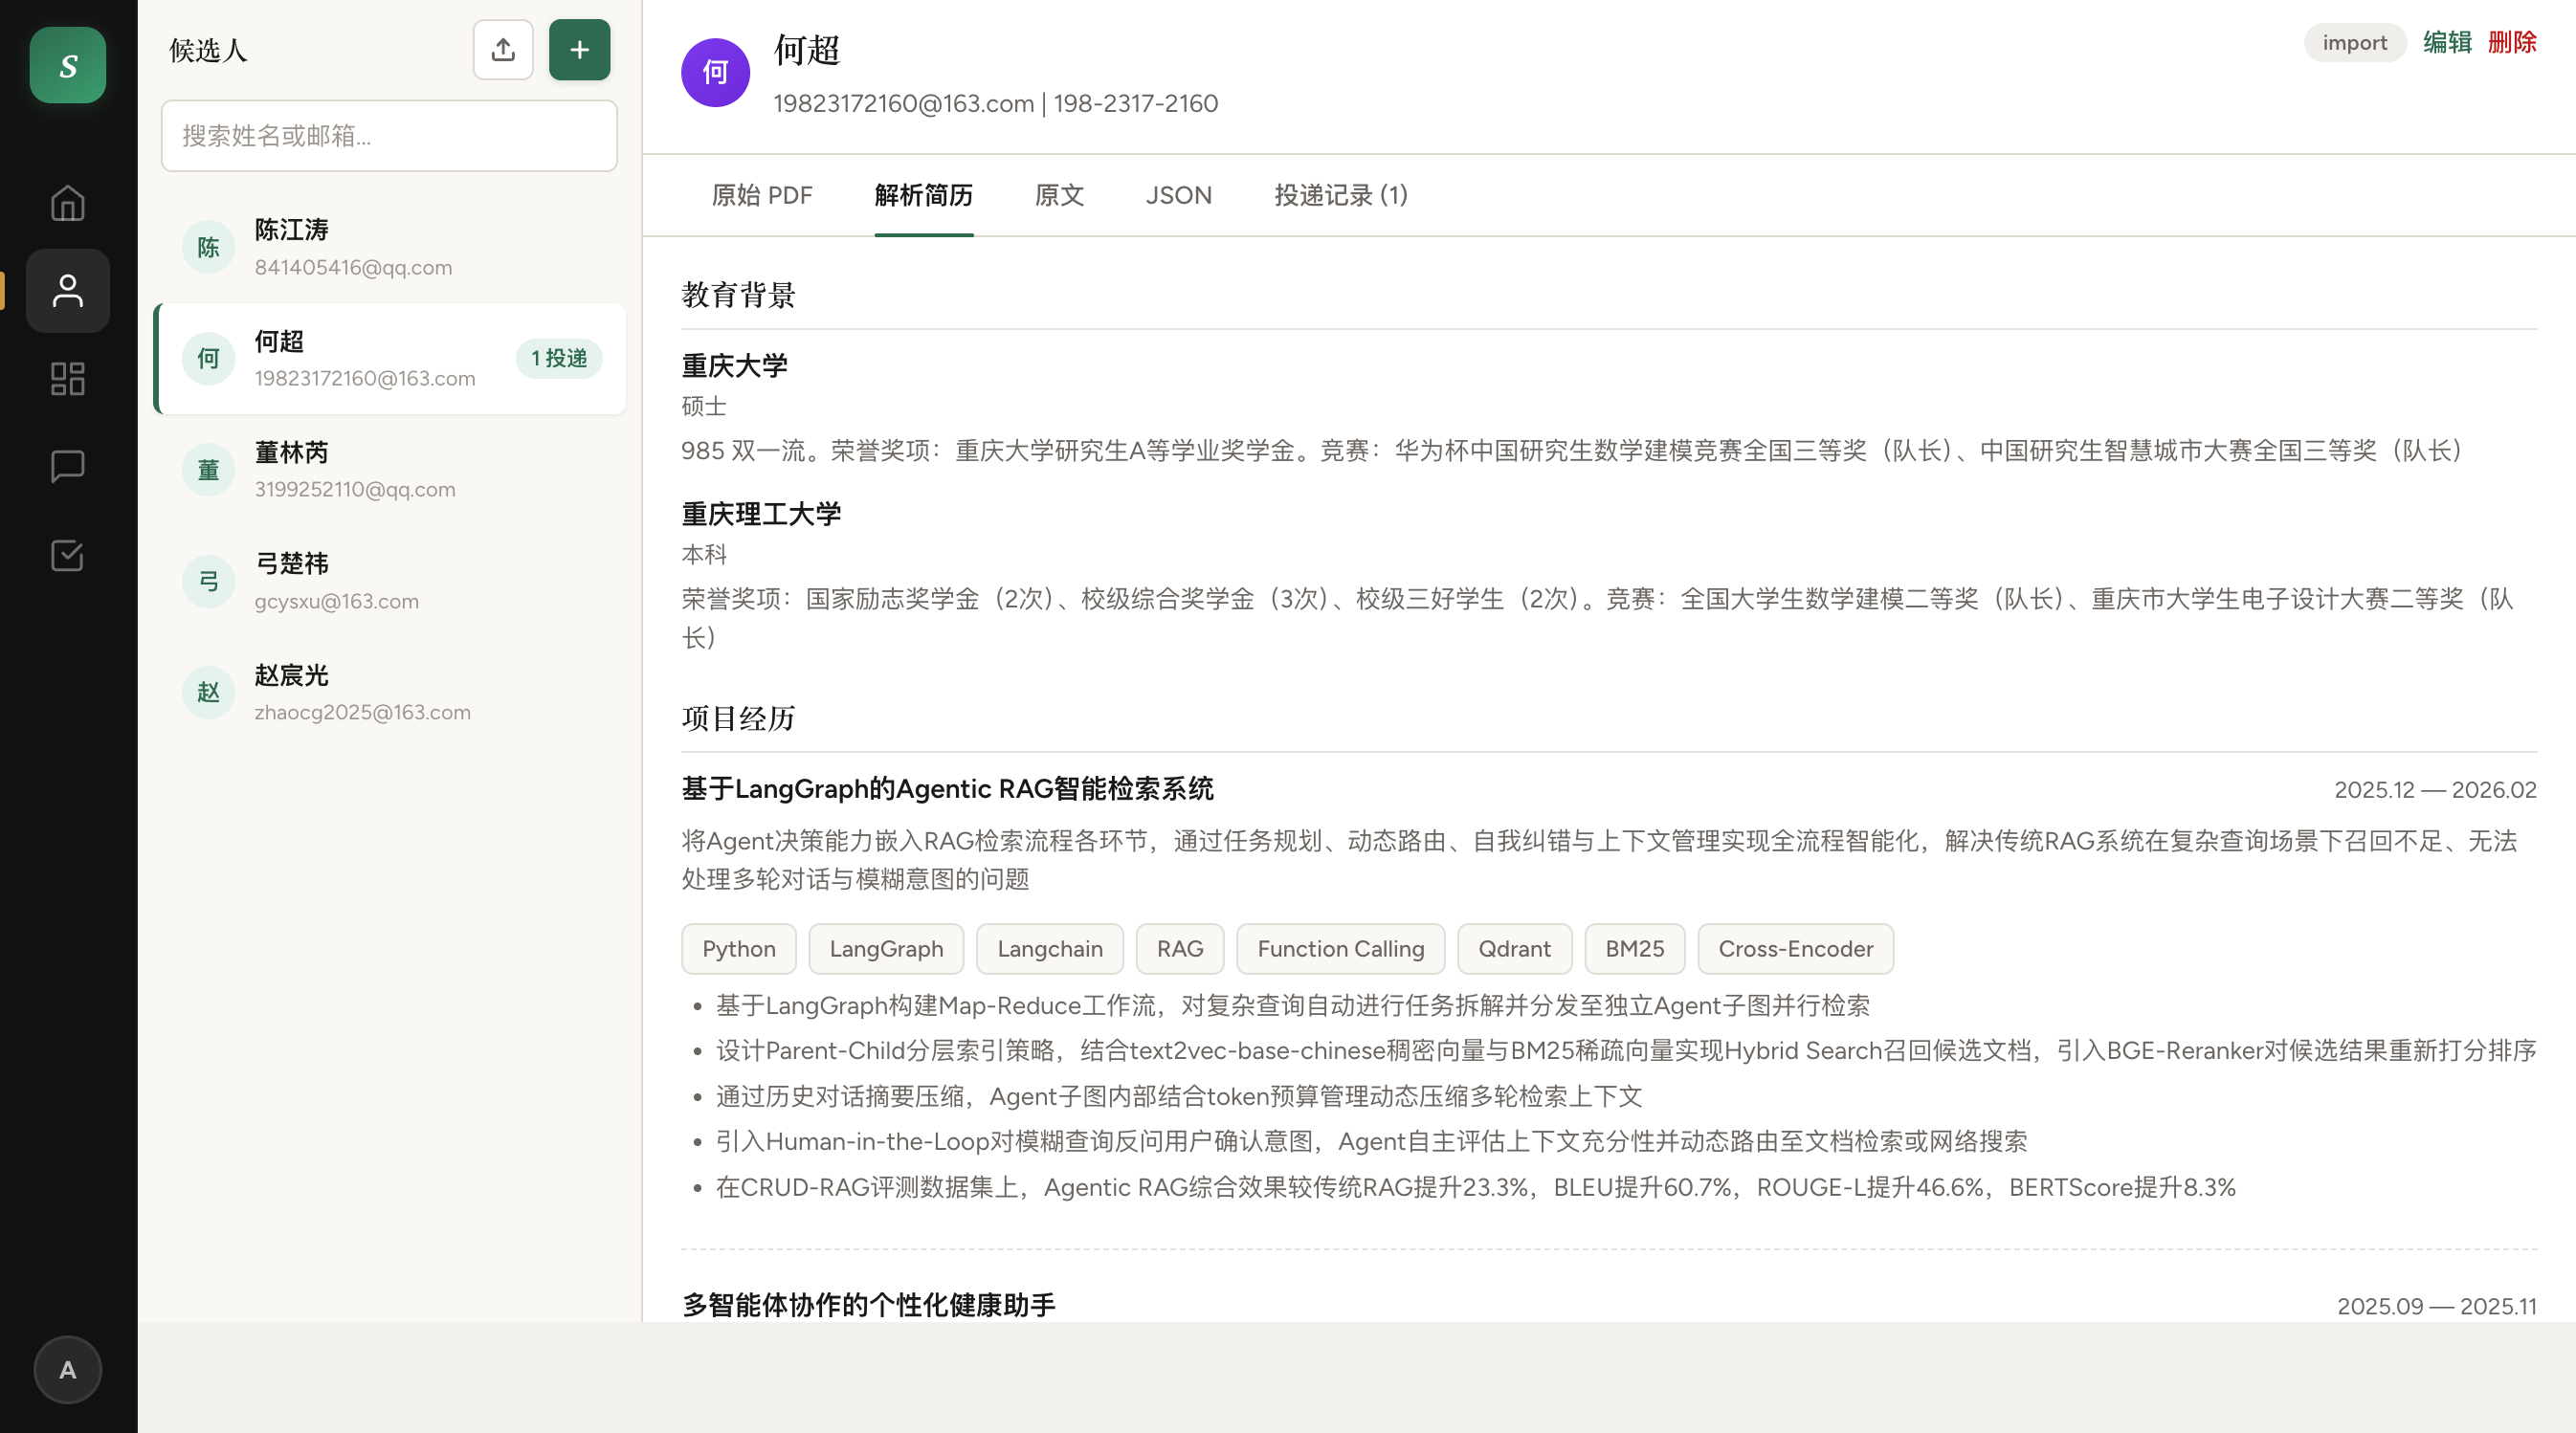
\includegraphics[width=0.96\textwidth]{media/candidate.png}
\caption{候选人库：简历全生命周期管理}
\label{fig:page-candidates}
\end{figure}

页面采用左右分栏布局。左栏提供候选人列表、实时搜索（按姓名/邮箱）、投递数量角标；右栏以多 Tab 形式展示候选人详情：

\begin{center}
\renewcommand{\arraystretch}{1.3}
\begin{tabular}{L{2.4cm} L{9.8cm}}
\toprule
\textbf{Tab} & \textbf{内容} \\
\midrule
原始 PDF & \texttt{fetchCVPdfBlob} 获取 Blob URL，iframe 全高预览；提供下载按钮 \\
解析简历 & 结构化渲染 \texttt{parsed\_json}：教育、工作经历（带职责要点）、项目、科研、技能标签 \\
原文 & 简历原始文本（\texttt{pre-wrap} 保留格式） \\
JSON & 树状递归展示 \texttt{parsed\_json} 完整结构，支持嵌套对象/数组 \\
投递记录 & 该候选人的所有投递（JD 名称、状态、匹配分、真实性分）及「前往评估助手」快捷跳转 \\
\bottomrule
\end{tabular}
\end{center}

简历上传后自动触发 \texttt{parseCV}，前端以 2 秒轮询感知解析进度；失败时显示错误信息并提供重试入口。

\subsection{企业与岗位工作台}

\begin{figure}[H]
\centering
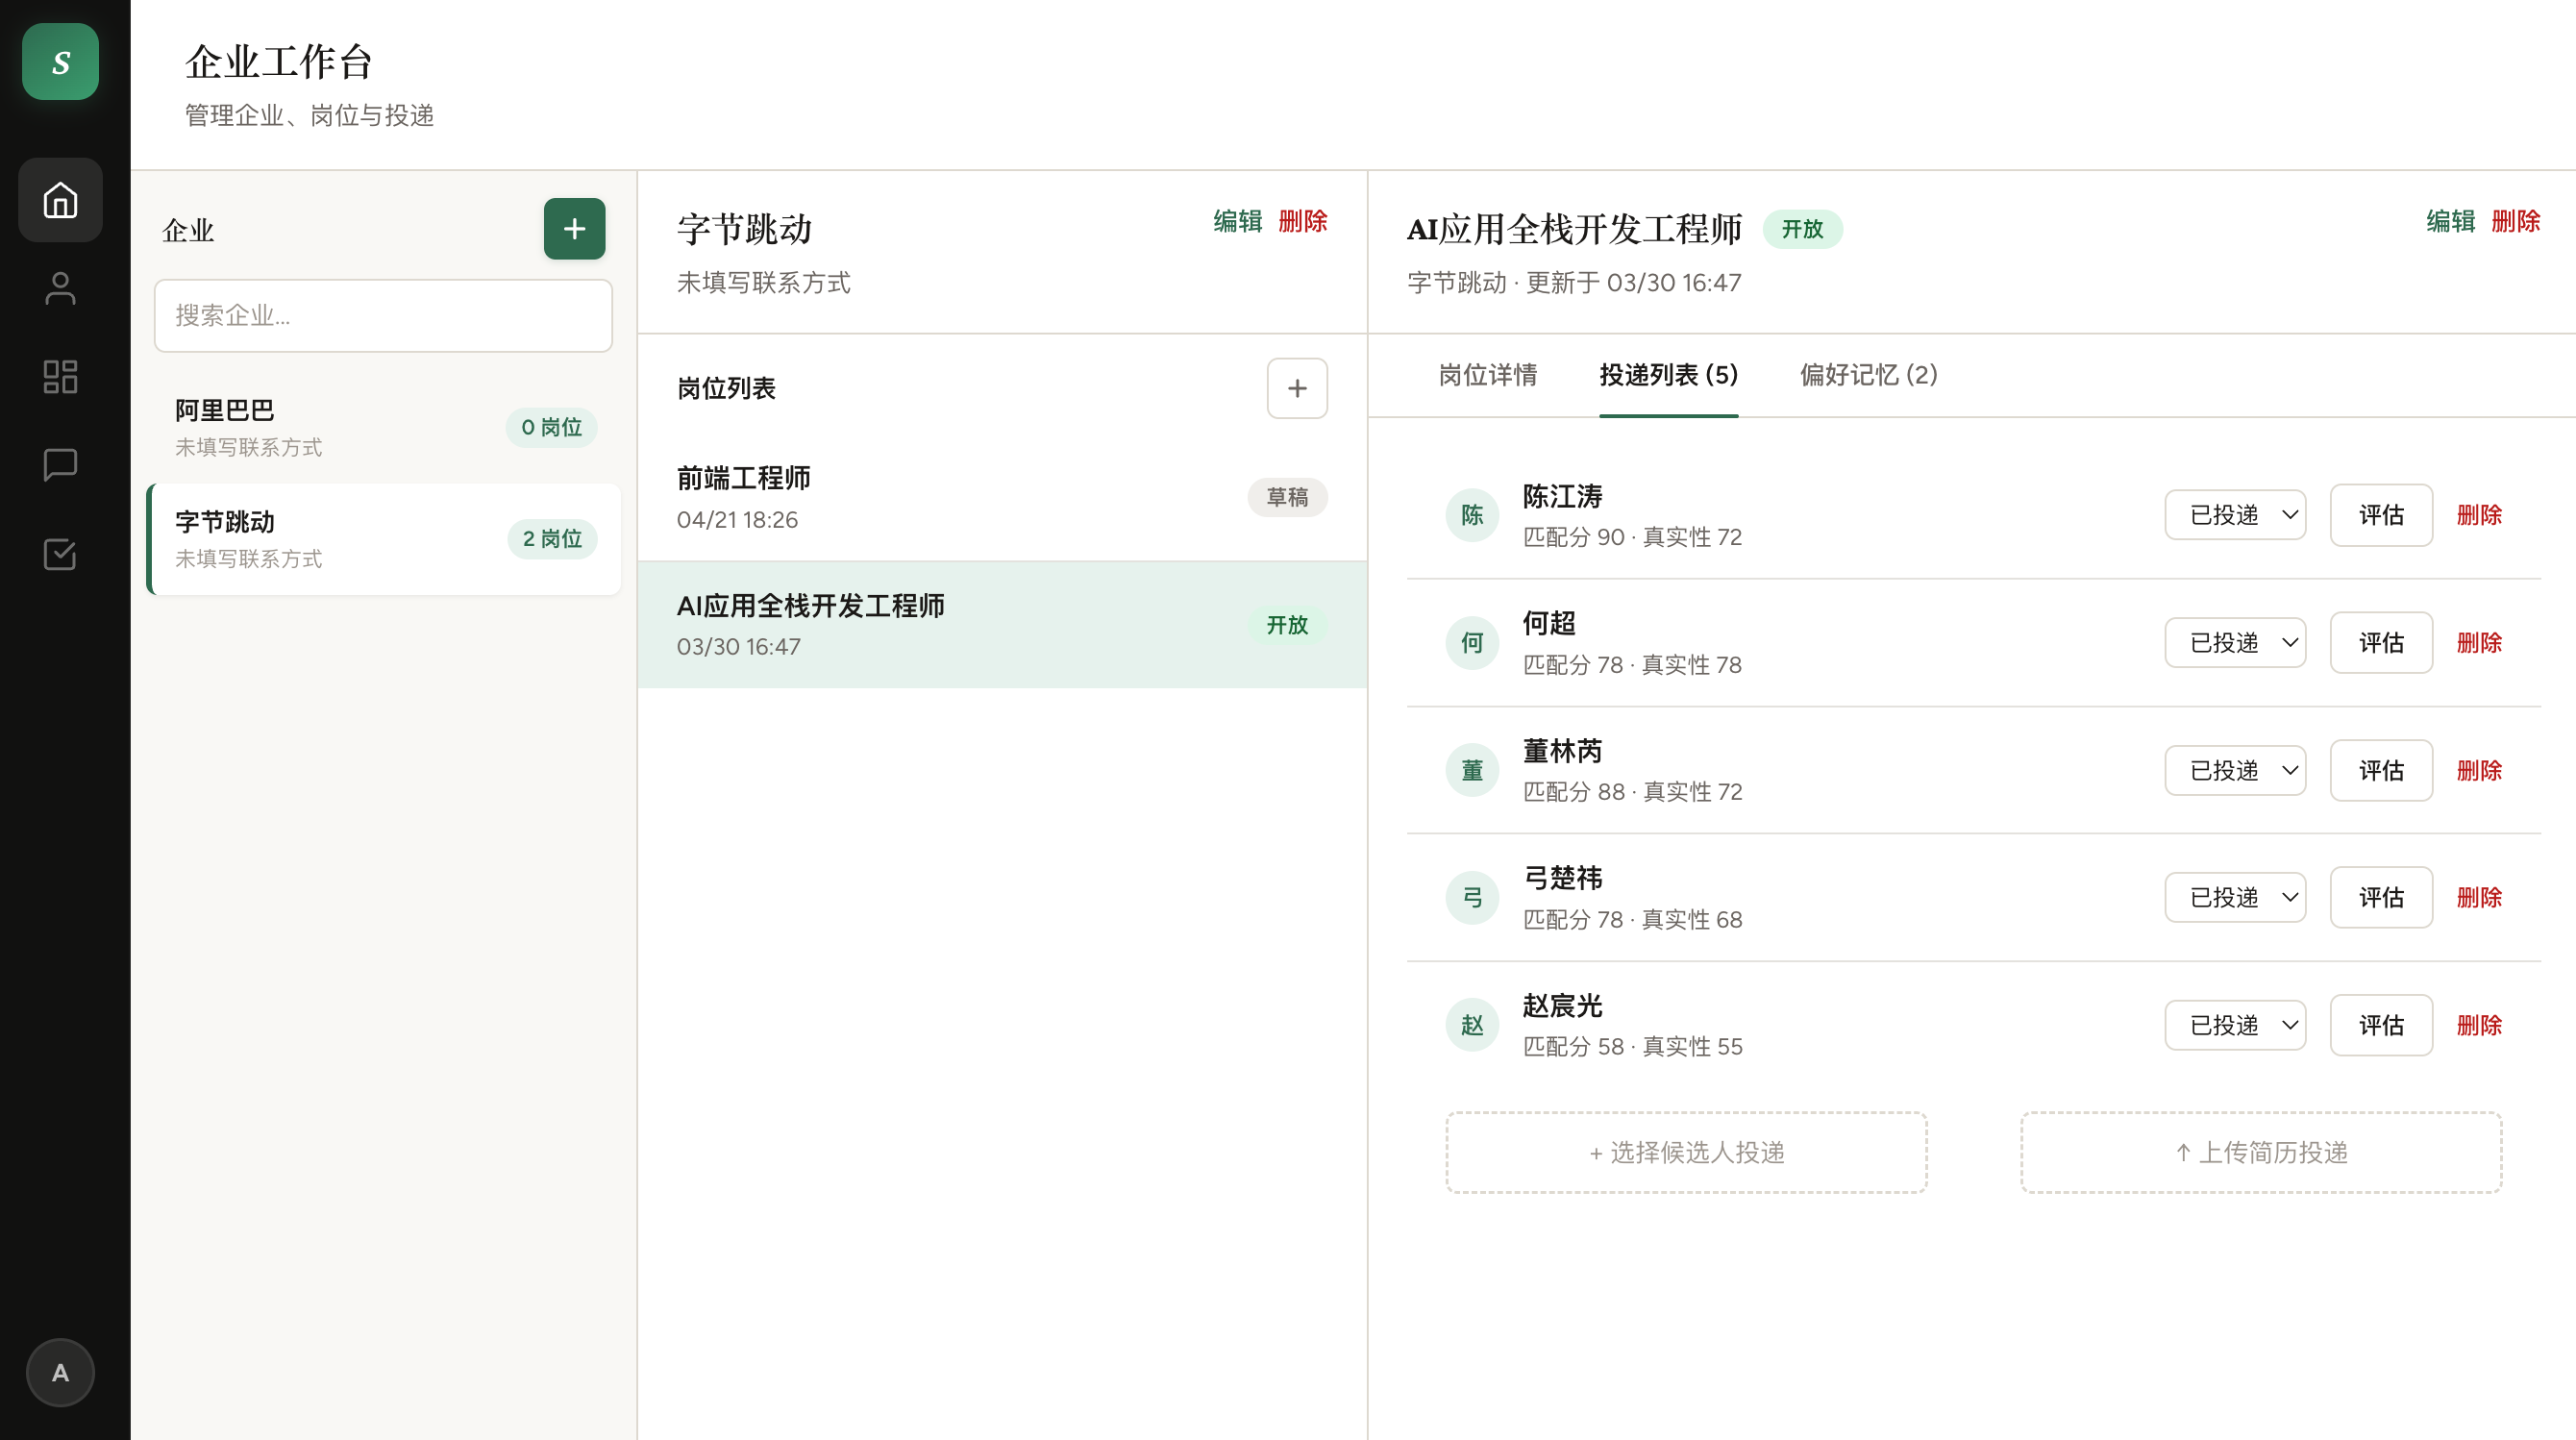
\includegraphics[width=0.96\textwidth]{media/enterprise.png}
\caption{企业与岗位工作台：三栏管理视图}
\label{fig:page-enterprise}
\end{figure}

页面采用三栏 \texttt{workspace-layout}：

\begin{itemize}[itemsep=3pt]
  \item \textbf{第一栏（企业列表）}：企业 CRUD，实时搜索，选中企业加载其岗位；
  \item \textbf{第二栏（岗位列表）}：在选中企业下创建/编辑/删除岗位，状态管理（\texttt{draft/open/closed}），角标显示投递数；
  \item \textbf{第三栏（岗位详情 Tab）}：「岗位信息」展示描述与要求；「投递列表」展示候选人、匹配分、真实性分、状态下拉；支持「从现有候选人选择」和「直接上传 PDF 自动建候选人+投递」两种新增投递方式；每行提供「前往评估助手」快捷跳转。
\end{itemize}

\subsection{评估看板}

\begin{figure}[H]
\centering
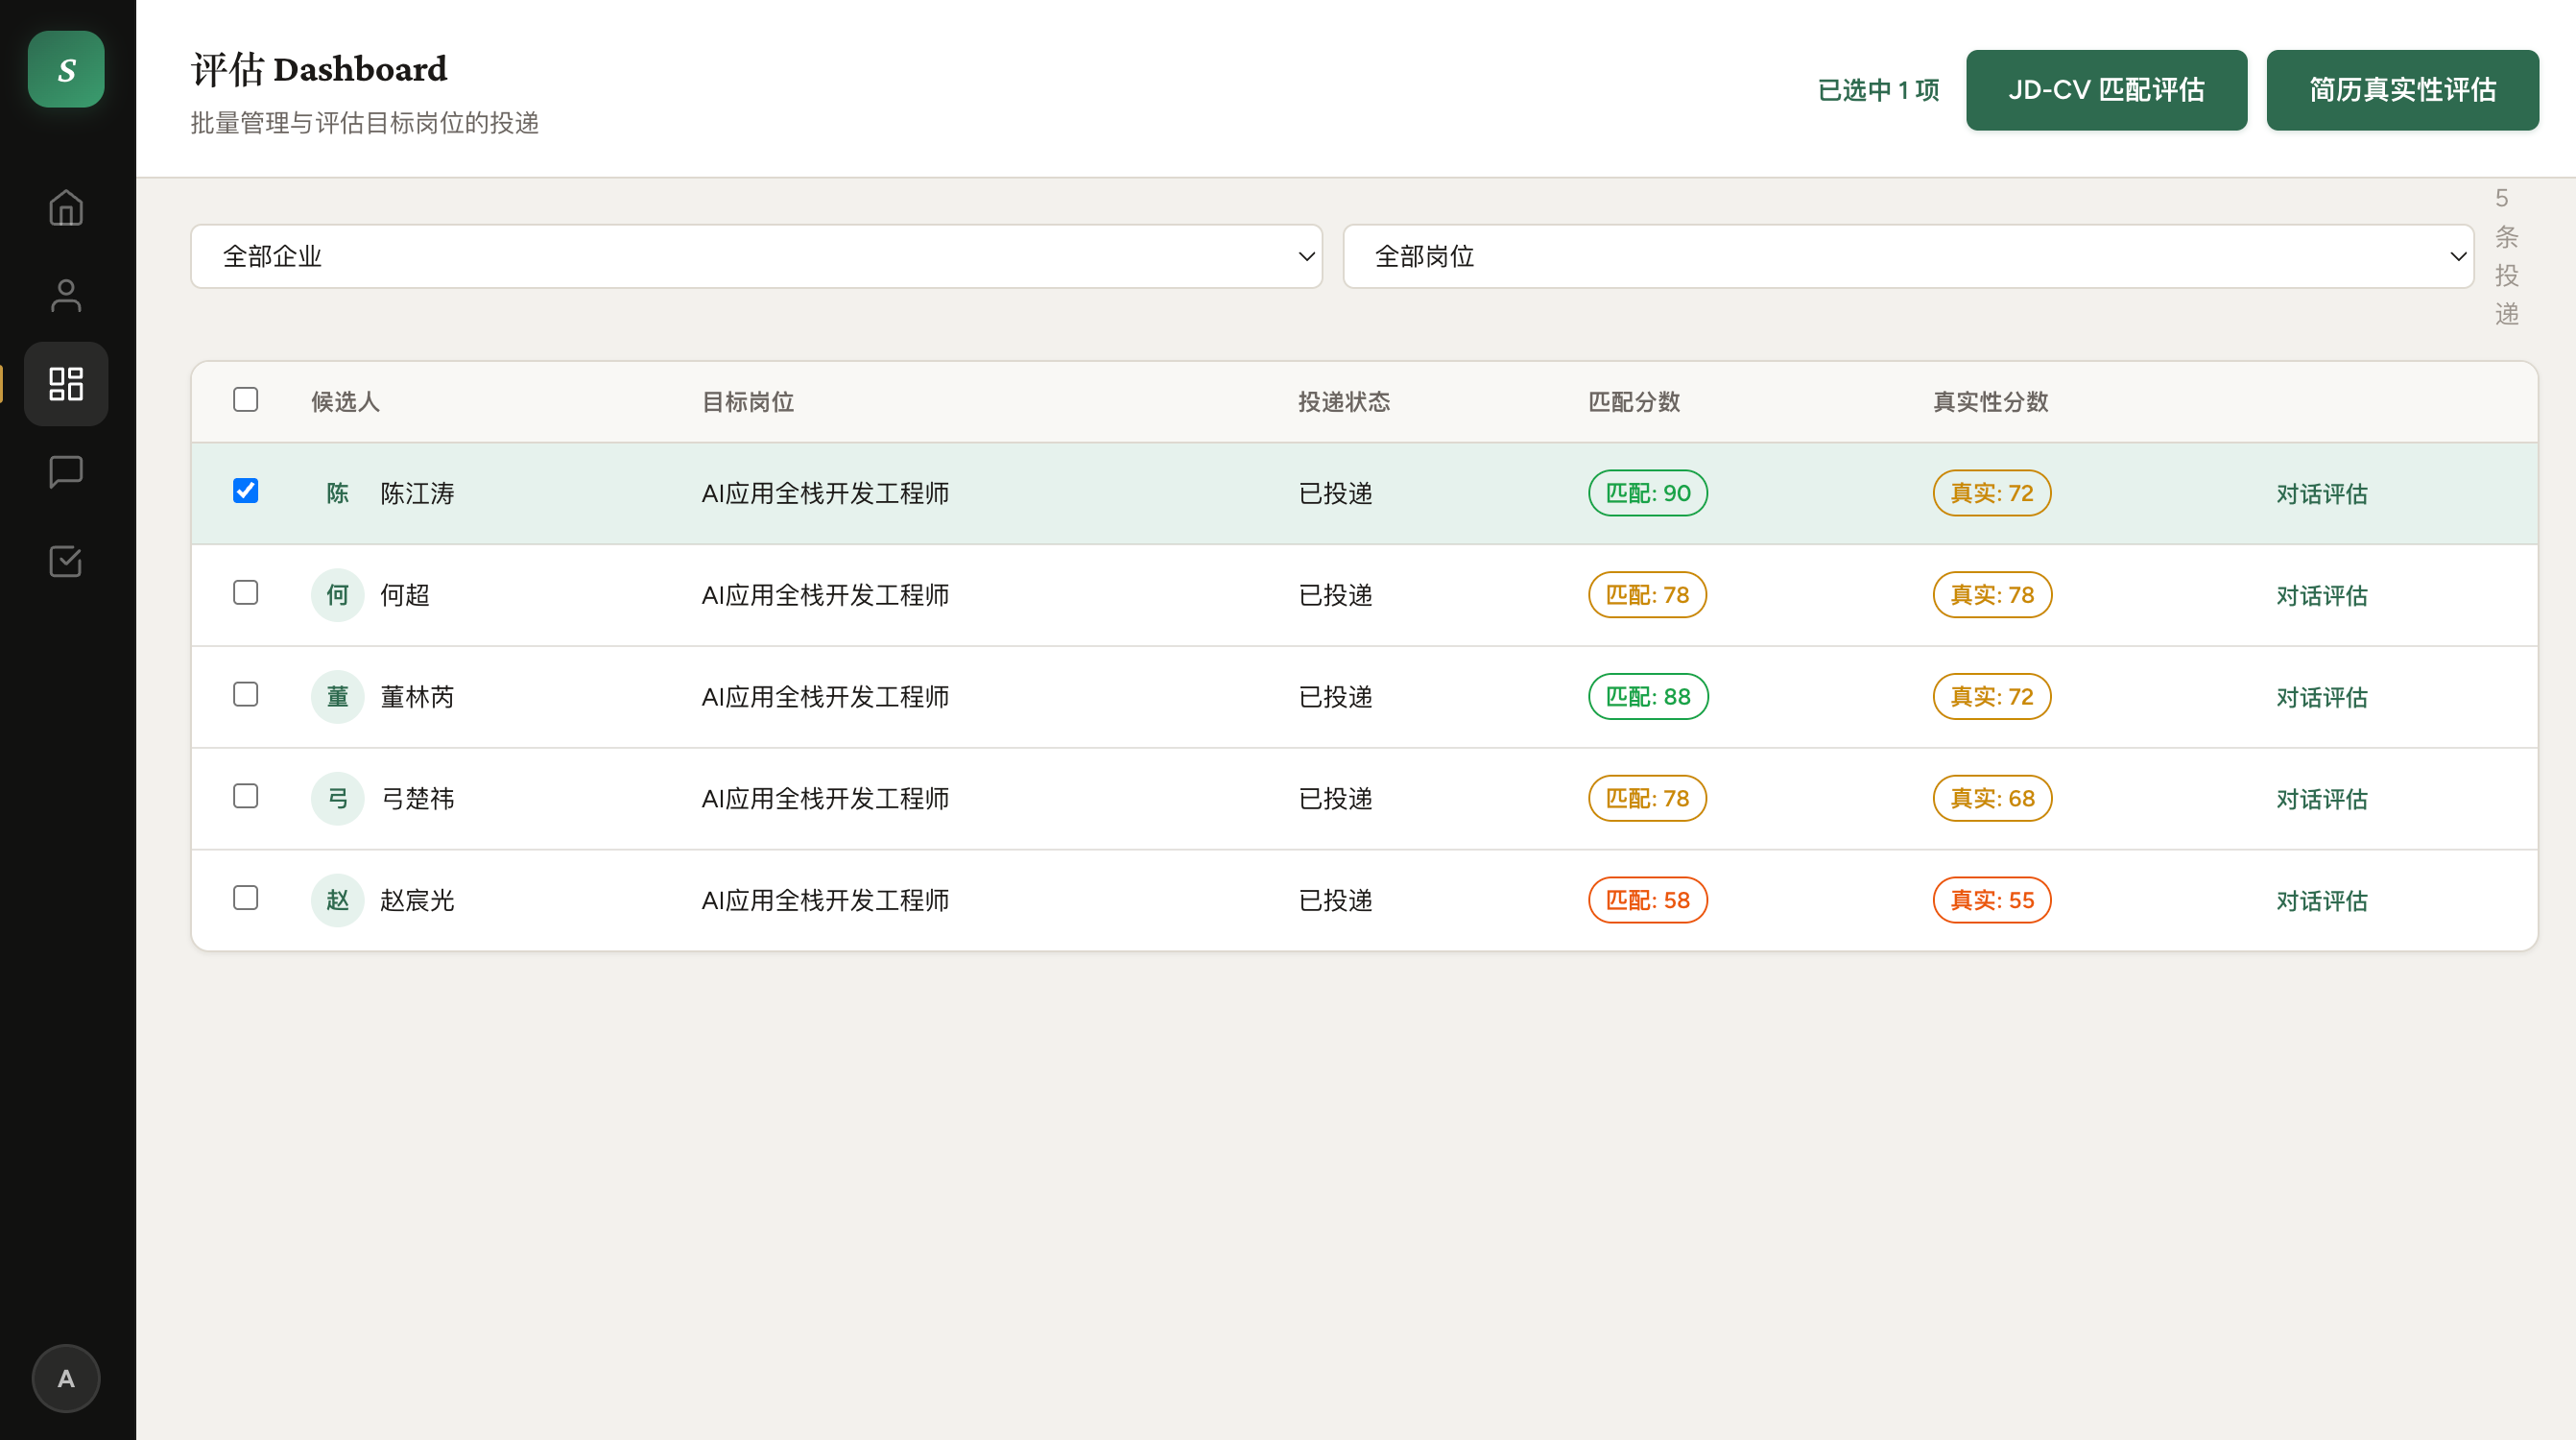
\includegraphics[width=0.96\textwidth]{media/dashboard.png}
\caption{评估看板}
\label{fig:page-dashboard}
\end{figure}

核心功能：
\begin{itemize}[itemsep=3pt]
  \item 企业 $\to$ 岗位二级联动筛选，定位目标投递集合；
  \item 多选投递后一键批量触发 JD-CV 匹配或真实性核查，请求间隔 1 秒保护 LLM 接口；
  \item \texttt{ScoreBadge}（颜色编码 + 档位字母）展示评估结果；点击分数弹出 \texttt{AssessmentReportModal}，含维度得分条（\texttt{DimensionBar}）、总结、优势/风险点列表。
\end{itemize}

\subsection{评估助手}

\begin{figure}[H]
\centering
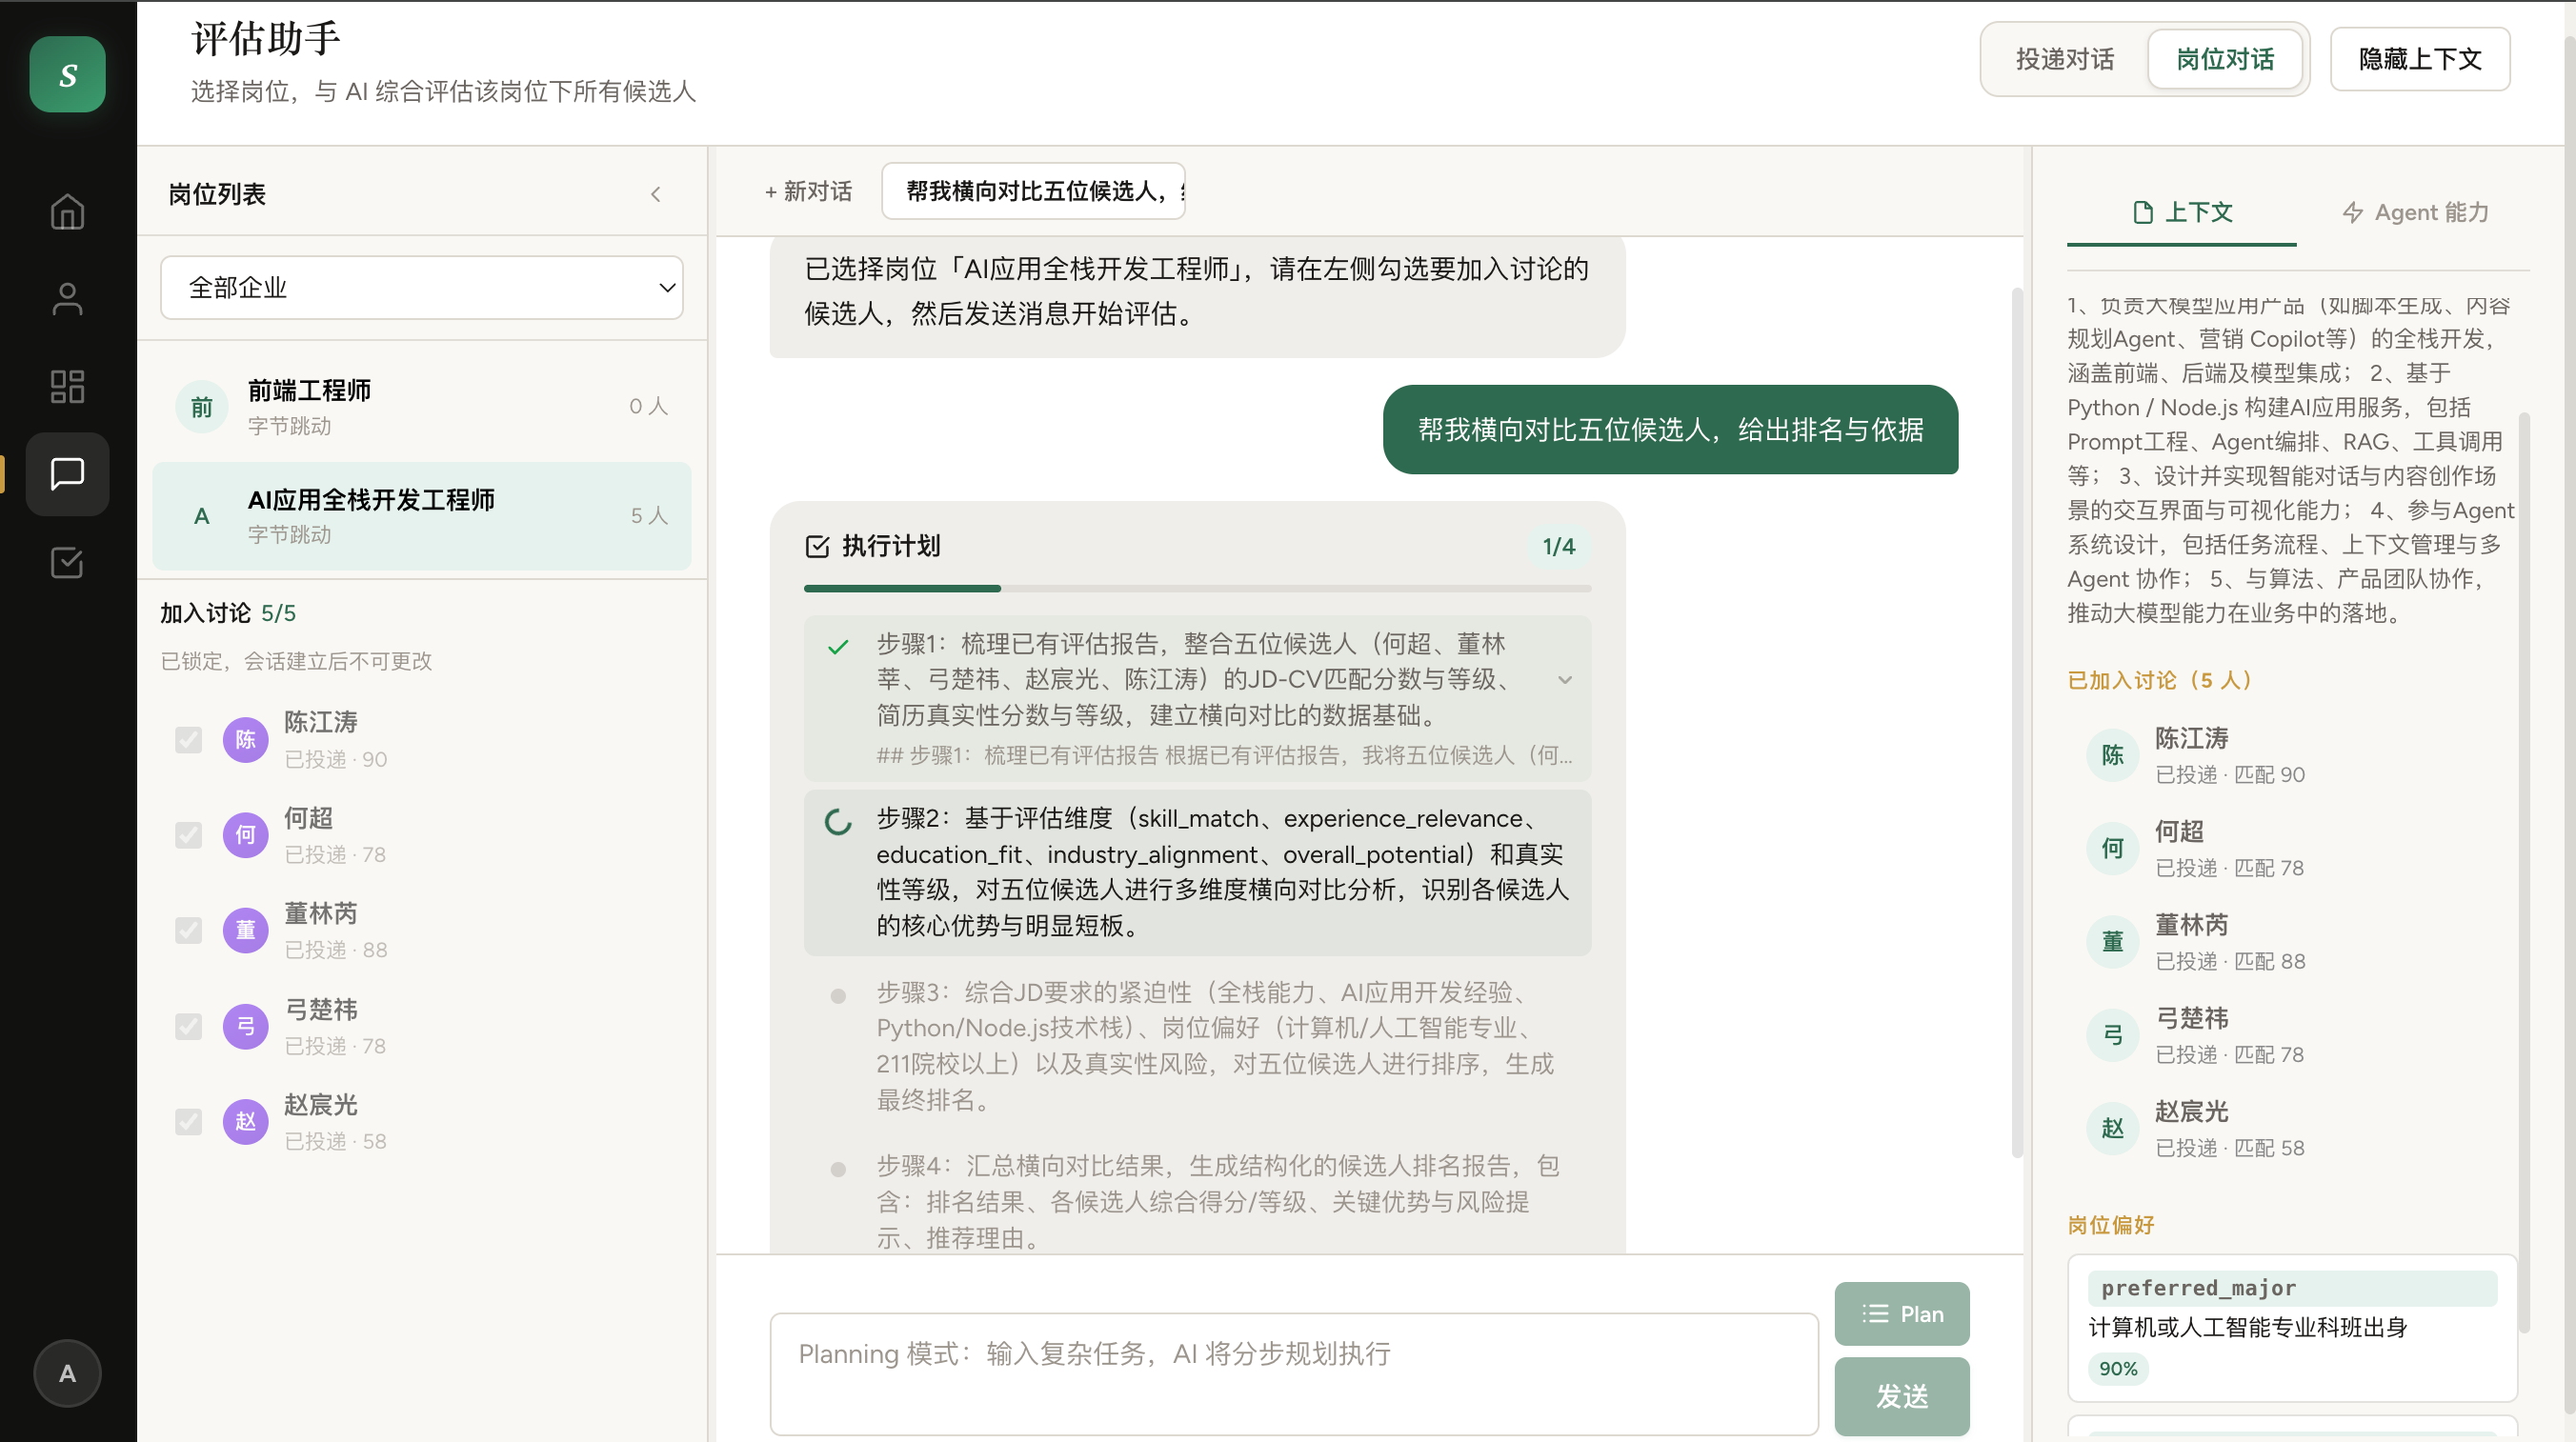
\includegraphics[width=0.96\textwidth]{media/assistant.png}
\caption{评估助手}
\label{fig:page-assistant}
\end{figure}

核心功能：
\begin{itemize}[itemsep=3pt]
  \item URL 参数 \texttt{?app=} 预选投递，自动拉取 JD、CV、历史评估上下文；
  \item Session Bar 管理多个历史会话，支持新建、切换和删除（\texttt{deleteChatSession}）；
  \item 对话使用 SSE 流式推理，\texttt{react-markdown + remark-gfm} 渲染 Markdown 响应；
  \item 右栏上下文面板：候选人信息摘要 + 岗位描述 + 投递状态与分数 + 可折叠评估报告卡；
  \item 左栏支持拖拽调整宽度与完全收起，最大化对话区面积。
\end{itemize}

% ==================================================
% 第五章 数据模型
% ==================================================
\section{数据模型}

\subsection{实体关系}

图~\ref{fig:er} 展示了系统核心实体之间的关系。

\begin{figure}[H]
\centering
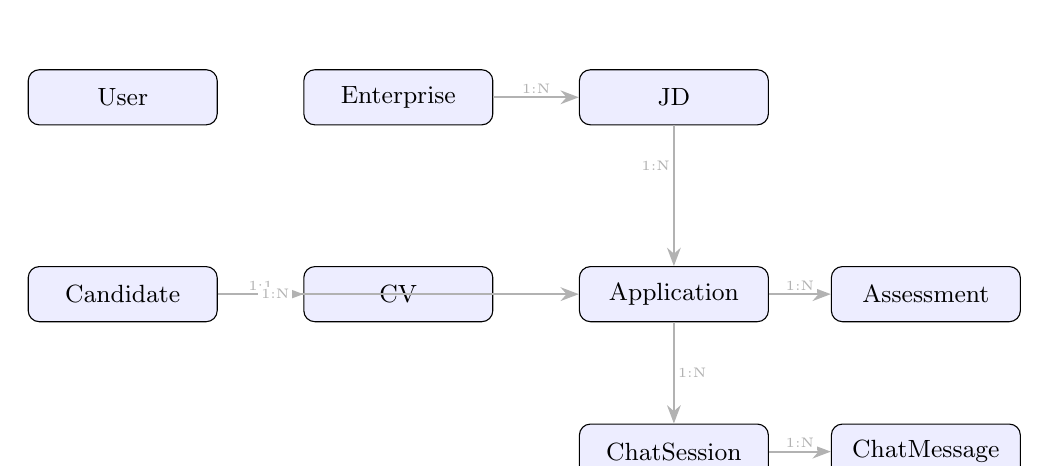
\begin{tikzpicture}[
  font=\small, >=Stealth,
  ent/.style={draw, rounded corners=4pt, fill=blue!7,
              minimum width=2.4cm, minimum height=0.7cm, text centered},
  rel/.style={font=\tiny, midway, fill=white, inner sep=1pt},
  arr/.style={thick, color=gray!60},
]
\node[ent] (user)  at (0,0)       {User};
\node[ent] (ent)   at (3.5,0)     {Enterprise};
\node[ent] (jd)    at (7,0)       {JD};
\node[ent] (cand)  at (0,-2.5)    {Candidate};
\node[ent] (cv)    at (3.5,-2.5)  {CV};
\node[ent] (app)   at (7,-2.5)    {Application};
\node[ent] (asmt)  at (10.2,-2.5) {Assessment};
\node[ent] (sess)  at (7,-4.5)    {ChatSession};
\node[ent] (msg)   at (10.2,-4.5) {ChatMessage};

\draw[arr,->] (ent) -- node[rel,above]{1:N} (jd);
\draw[arr,->] (cand) -- node[rel,above]{1:1} (cv);
\draw[arr,->] (cand.east) -- ++(0.5,0) |- node[rel,right]{1:N} (app.west);
\draw[arr,->] (jd.south) -- ++(0,-0.4) -| node[rel,below left]{1:N} (app.north);
\draw[arr,->] (app) -- node[rel,above]{1:N} (asmt);
\draw[arr,->] (app.south) -- node[rel,right]{1:N} (sess.north);
\draw[arr,->] (sess) -- node[rel,above]{1:N} (msg);
\end{tikzpicture}
\caption{核心数据模型 ER 图}
\label{fig:er}
\end{figure}

\subsection{核心表字段摘要}

\begin{center}
\renewcommand{\arraystretch}{1.3}
\begin{tabular}{L{2.6cm} L{9.8cm}}
\toprule
\textbf{表} & \textbf{关键字段} \\
\midrule
\texttt{user} & \texttt{username}, \texttt{email}, \texttt{password\_hash}, \texttt{user\_type} \\
\texttt{enterprise} & \texttt{name}, \texttt{industry}, \texttt{description} \\
\texttt{jd} & \texttt{enterprise\_id}, \texttt{title}, \texttt{description}, \texttt{requirements\_text}, \texttt{parsed\_json}, \texttt{status} \\
\texttt{candidate} & \texttt{name}, \texttt{email}, \texttt{phone}, \texttt{source} \\
\texttt{cv} & \texttt{candidate\_id}, \texttt{raw\_text}, \texttt{parsed\_json}, \texttt{file\_data}, \texttt{file\_name}, \texttt{parse\_status}, \texttt{parse\_error} \\
\texttt{application} & \texttt{candidate\_id}, \texttt{jd\_id}, \texttt{status}, \texttt{latest\_match\_score}, \texttt{latest\_authenticity\_score} \\
\texttt{assessment} & \texttt{application\_id}, \texttt{assessment\_type}, \texttt{score}, \texttt{level}, \texttt{summary}, \texttt{result\_json} \\
\texttt{chat\_session} & \texttt{application\_id}, \texttt{jd\_id}, \texttt{scope}, \texttt{title} \\
\texttt{chat\_message} & \texttt{session\_id}, \texttt{role}, \texttt{content}, \texttt{metadata\_json} \\
\bottomrule
\end{tabular}
\end{center}

% ==================================================
% 第六章 技术栈汇总
% ==================================================
\section{技术栈汇总}\label{sec:techstack}

\begin{center}
\renewcommand{\arraystretch}{1.35}
\begin{tabular}{L{2.8cm} L{4.5cm} L{5.4cm}}
\toprule
\textbf{层} & \textbf{技术} & \textbf{说明} \\
\midrule
前端框架 & React 18 + TypeScript & 组件化 UI \\
前端路由 & React Router v7 & SPA 路由管理 \\
前端构建 & Vite 5 & 开发服务器与构建优化 \\
Markdown 渲染 & react-markdown + remark-gfm & 对话消息 Markdown 渲染 \\
后端框架 & FastAPI（Python 3.13） & REST API + SSE 流式接口 \\
ORM & SQLAlchemy & 数据库访问层 \\
数据库 & PostgreSQL 16 & 主数据存储 \\
迁移 & Alembic & 数据库版本管理 \\
LLM 框架 & LangChain + LangGraph & Agent 编排与对话流 \\
LLM 接口 & OpenAI 兼容 API（Kimi K2.5） & 语言模型调用，主备容错 \\
对话持久化 & langgraph-checkpoint-postgres & 会话状态持久化 \\
知识图谱 & Neo4j + Python 驱动 & 技能图谱查询 \\
PDF 解析 & PyMuPDF & PDF 文本抽取 \\
认证 & PyJWT & JWT Token 鉴权 \\
容错重试 & tenacity & LLM 调用自动重试 \\
容器化 & Docker Compose & PostgreSQL 容器管理 \\
\bottomrule
\end{tabular}
\end{center}

% ==================================================
% 第七章 服务部署与运行环境
% ==================================================
\section{服务部署与运行环境}

\subsection{云主机与操作系统}

本系统部署在\textbf{阿里云弹性计算服务（ECS）}上，实例规格为 \textbf{2 核 CPU / 2\,GB 内存}（可按业务负载后续升配）。宿主机操作系统采用 \textbf{Ubuntu Server 22.04 LTS}（x86\_64），便于使用官方 Docker 源、长期安全更新以及与课程/文档环境一致。

公网访问通过阿里云分配的弹性公网 IP 绑定至该实例，当前站点入口为 \url{http://8.130.114.230/}（可按需改为域名并配置 HTTPS 证书）。

\subsection{宝塔面板与 Web 入口}

\textbf{Nginx}、站点、SSL 证书及反向代理规则等通过\textbf{宝塔 Linux 面板}（BT Panel）进行可视化管理与下发：在面板中创建网站、指向前端构建产物目录，并将 \texttt{/api}（或后端实际前缀）代理到本机 \textbf{Uvicorn} 监听的 FastAPI 端口，从而避免手工编辑大量 Nginx 配置片段、降低运维出错率。宝塔同时便于查看进程、日志与防火墙端口放行，与 Ubuntu 上自行安装的 Docker、Python 运行环境并行使用。

\subsection{服务拓扑与端口}

\begin{figure}[H]
\centering
\resizebox{0.98\textwidth}{!}{%
\begin{tikzpicture}[
  font=\small, >=Stealth,
  inet/.style={draw, rounded corners=4pt, fill=blue!8, align=center, minimum width=2.5cm, minimum height=0.75cm},
  box/.style={draw, rounded corners=3pt, fill=white, align=center, minimum width=2.85cm, minimum height=0.72cm},
  arr/.style={->, thick, color=gray!60},
]
% 纵向分层；主业务 / 环回 / AutoDL 水平间距加大，避免框体重叠（单位：cm）
\node[inet] (net) at (0,0) {Internet};
\node[font=\footnotesize\itshape, anchor=east, align=right] at (-3.2,-0.95)
  {Ubuntu 22.04 LTS · 2核4GB};

\node[box, fill=yellow!12] (bt) at (-6.2,-3.4) {宝塔面板\\运维入口};
\node[box, fill=orange!10] (nx) at (0,-3.4) {Nginx\\:80 / :443};

\node[box, fill=blue!8] (fe) at (-6.2,-6.2) {静态资源\\Vite build};
% 主业务略左移，环回与 AutoDL 右移，保证与 be 东缘、彼此之间有足够间隙
\node[box, fill=blue!8, minimum width=3.0cm] (be) at (-0.85,-6.2) {主业务后端\\Uvicorn :8000};
\node[draw, rounded corners=3pt, fill=gray!12, align=center, font=\footnotesize,
      minimum width=2.5cm, minimum height=0.95cm, inner sep=3pt] (loc) at (4.15,-6.2)
  {\texttt{127.0.0.1:9000}\\[-2pt]\tiny 本机环回};
\node[draw, dashed, rounded corners=6pt, fill=red!7, align=center, inner sep=5pt,
      minimum width=3.6cm, minimum height=1.5cm] (adl) at (9.85,-6.2)
  {\textbf{AutoDL}\\[1pt]FastAPI \texttt{:8000} · \texttt{/predict}\\[1pt]\footnotesize Qwen · RTX 5090};

\node[box, fill=green!8, minimum width=2.55cm] (pg) at (-3.4,-9.2) {PostgreSQL\\:5432};
\node[box, fill=green!8, minimum width=2.55cm] (nj) at (3.4,-9.2) {Neo4j\\:7687};

% Internet → Nginx
\draw[arr] (net.south) -- (0,-0.55);
\draw[arr] (0,-0.55) -- (0,-1.85) -- (nx.north);

% 宝塔 ↔ Nginx
\draw[arr, dashed, color=gray!45] (bt.east) -- node[above,font=\tiny,yshift=2pt]{运维配置} (nx.west);

% Nginx → 静态 / 后端：一律接入矩形「上沿中点」(north)，先共线下垂再分开，避免短线交叉
% split 位于 Nginx 与下一行之间；到静态为「横移 + 竖落到 fe.north」；到后端为纯竖线
\coordinate (nxsplit) at (0,-5.05);
\draw[arr] (nx.south) -- (nxsplit);
% 静态：长水平段后落到 fe.north，标签放在水平段下方
\draw[arr] (nxsplit) -| node[pos=0.42, below, font=\tiny, yshift=-1pt]{站点根} (fe.north);
% 后端：竖直连到 be.north
\draw[arr] (nxsplit) -- node[right, font=\tiny, xshift=4pt]{反代} (be.north);

% 后端 → 数据库：分叉点对齐主业务中心
\coordinate (dbfork) at (-0.85,-7.35);
\draw[arr] (be.south) -- (dbfork);
\draw[arr] (dbfork) -| (pg.north);
\draw[arr] (dbfork) -| (nj.north);

% 主业务 → 环回 → AutoDL（标签缩短，命令见正文）
\draw[arr] (be.east) -- node[above, font=\tiny, yshift=2pt]{HTTP} (loc.west);
\draw[arr, dashed, color=purple!55, thick] (loc.east) --
  node[above, font=\scriptsize, yshift=3pt]{SSH 转发} (adl.west);
\end{tikzpicture}%
}
\caption{部署拓扑：Web、数据库与 AutoDL 推理（SSH 端口转发）}
\label{fig:deploy-topo}
\end{figure}

图~\ref{fig:deploy-topo} 示意\textbf{Web 与数据层}及\textbf{AutoDL Qwen 推理}：经 \textbf{Nginx} 访问静态与主业务 \textbf{Uvicorn}；\textbf{PostgreSQL} / \textbf{Neo4j} 在宿主机容器内运行。过度包装等推理由主业务访问 \texttt{127.0.0.1:9000}，再经 \textbf{SSH} 转发至 AutoDL 上 FastAPI（RTX 5090）。其余云端 LLM 走公网 HTTPS，图中未画。

\subsection{大模型推理服务（AutoDL 与 SSH 端口转发）}

面向\textbf{简历过度包装倾向}等需要可控、可复现推理的评估环节，本系统采用\textbf{通义千问（Qwen）}模型；推理服务部署在\textbf{AutoDL} 租用的 GPU 实例上，显存环境为 \textbf{NVIDIA RTX 5090}。在 AutoDL 机器上以独立 \textbf{FastAPI} 进程加载模型并对外提供 HTTP 接口（实例内监听 \texttt{127.0.0.1:8000}，路由示例为 \texttt{/predict}，以实际代码为准）。

阿里云 ECS 仅 \textbf{2\,GB 内存}，不适合在站内直接加载 7B/14B 级权重做 GPU/CPU 推理：CPU 推理极慢且易 \textbf{OOM}；将推理与站点解耦，可按任务时段租用 AutoDL 算力，避免为整站长期绑定高价 GPU 实例。

站点服务器（ECS）与 AutoDL 之间通过 \textbf{SSH 本地端口转发} 将远端 FastAPI 映射到 ECS 本机环回地址，典型命令为：

\begin{center}
\texttt{ssh -L 9000:127.0.0.1:8000 root@<AutoDL\_实例公网或可 SSH 的地址>}
\end{center}

隧道建立后，主业务后端在 ECS 上访问 \texttt{http://127.0.0.1:9000/predict}，即可转发到 AutoDL 上 \texttt{8000} 端口的推理服务（若本地改用其他本地端口，将 \texttt{9000} 换成实际绑定端口即可）。生产环境可使用 \texttt{autossh} 或在 \texttt{systemd} 中注册服务以保持隧道自动重连；AutoDL 实例重建或更换 IP 时，需同步更新 SSH 目标与防火墙策略。

\textbf{说明}：其他智能体（如 JD-CV 匹配、深度对话）若仍通过 OpenAI 兼容接口调用云端大模型（如 Kimi），与上述\textbf{自托管 Qwen 推理}路径可并行存在，在 \texttt{.env} 中分别配置 Base URL 即可。

\subsection{启动与配置}

\begin{itemize}[itemsep=4pt]
  \item \textbf{数据库}：用容器编排启动 PostgreSQL，Neo4j 可同组或独立容器；端口在云厂商安全组与宝塔防火墙中一致放行。
  \item \textbf{后端}：Python 3.13 虚拟环境中安装依赖，执行 \texttt{alembic upgrade head} 迁移后，以 \texttt{uvicorn app.main:app --host 0.0.0.0 --port 8000} 启动；生产环境可配合 \texttt{systemd} 或宝塔「Python 项目管理器」等守护进程方式常驻。
  \item \textbf{大模型 SSH 隧道}：先建立至 AutoDL 的转发并确认本机 \texttt{127.0.0.1:9000} 上推理接口可达，应用配置中对应 Base URL 指向该地址；隧道未建立时相关调用会失败。
  \item \textbf{前端}：构建静态文件至 \texttt{dist/}，在宝塔站点中配置网站根目录指向该目录；Nginx 反代规则可在面板「反向代理」中维护。开发阶段仍可在本地 \texttt{npm run dev} 调试。
  \item \textbf{环境变量}：在服务器 \texttt{.env} 或宝塔「环境变量」/密钥管理中配置数据库连接串、\texttt{JWT\_SECRET}、Neo4j 连接、云端 LLM 的 \texttt{OPENAI\_API\_KEY} / Base URL，以及\textbf{自托管 Qwen 推理服务}的 URL（如 \texttt{http://127.0.0.1:9000}）等，\textbf{严禁}将密钥、SSH 私钥与 AutoDL 登录信息提交至版本库。
\end{itemize}

\end{document}
